

\chapter{Social engineering and AI\label{chapter:background}}
\begin{comment}
- osakysymykset?
- vertailukohteet?
- cost-benefit ratio johonkin kohtaan?
\end{comment}


%
% Generative AI in SE, chapter overview
%
In recent years, the integration of generative artificial intelligence (AI) into social engineering offensive practices has emerged as a significant concern within the field of cybersecurity~\citep{blauth_AI_Crime_Overview_Malicious_Use_Abuse_2022, king_AI_Crime_Interdisciplinary_Analysis_2019, mirsky_Threat_Offensive_AI_Organizations_2023}. This chapter provides an overview of the role of generative AI in social engineering and explains the key concepts of open-source intelligence, AI, and generative AI.

%After this, Chapter~\ref{chapter:attacks} examines generative AI -powered social engineering attack vectors and tools.



%
% Defining social engineering
%
A consensus regarding the strict definition of social engineering is lacking in the field~\citep{hatfield_SE_Evolution_Concept_2018}. For the purposes of this thesis, social engineering is defined as "\textit{a type of attack wherein the attacker(s) exploit human vulnerabilities by means of social interaction to breach cybersecurity, with or without the use of technical means and technical vulnerabilities}"~\citep{wang_Defining_Social_Engineering_2020}.



%
% Cybersecurity threats to organizations
%
Today, organizations confront cybersecurity threats from a range of sources, including cybercriminals, disgruntled or malicious employees, amateur hackers, hacktivists, competitors, and even state-sponsored cyber terrorists~\citep{mirsky_Threat_Offensive_AI_Organizations_2023}. These threat actors may be driven by motives such as financial gain, intellectual property theft, sabotage, fame, or revenge. Organizations face public scrutiny, loss of customer trust and relations, governmental penalties, and loss of productivity, among other things, due to data breaches. With the annual average cost of a data breach reaching \$4,88 million~\citep{ibm_Cost_Data_Breach_Report_2024}, and cybercrime-related losses steadily increasing~\citep{verizon_Data_Breach_Investigations_Report_2024}, organizations need to take precautions to protect their data and other assets.


%
% Why these attack vectors were chosen and not some others
%
While the field of social engineering contains many attack vectors, not all of them are amiable to be enhanced by AI technologies directly. Research literature has identified and primarily focused on three distinct, but closely related, AI-powered attack vectors: spear phishing~\citep{basit_Comprehensive_Survey_AI_Phishing_Detection_2021}, impersonation utilizing deepfakes~\citep{mirsky_Creation_Detection_Deepfakes_2021}, and real-time voice morphing~\citep{doan_BTSE_Audio_Deepfake_Detection_2023}. Other popular social engineering attack methods, which do not directly benefit from the advancement of AI technologies, and which are thus not addressed in this thesis, include dumpster diving and shoulder surfing~\citep{mirsky_Threat_Offensive_AI_Organizations_2023}. Table \ref{table:attacks} briefly explains some of the most common social engineering attack vectors. Ransomware attacks are listed as an example of a social engineering attack which can be amplified by AI directly but which isn’t, due to its different nature, examined in this thesis.

\begin{table}[ht!]  
\centering  
\renewcommand{\arraystretch}{1.5} % Adjust row height for better readability  
\setlength{\tabcolsep}{5pt} % Adjust column spacing  
\begin{tabularx}{\textwidth}{|l|X|l|l|} % X column for text wrapping  
\hline  
\textbf{Attack vector} & \textbf{Brief description} & \textbf{Relevance} & \textbf{Included} \\ \hline  
Dumpster diving & Going through someone's trash for sensitive information & No & No \\ \hline  
Impersonation & Claiming to be someone else & Yes & Yes \\ \hline  
Phishing & Deceptive attempts to steal sensitive information & Yes & Yes \\ \hline  
Ransomware & Locking the victim's data against a ransom payment or other action & Yes & No \\ \hline  
Shoulder surfing & Covertly observing people enter sensitive information such as login details & No & No \\ \hline  
Spear phishing & A targeted variety of phishing & No & Yes \\ \hline  
\end{tabularx}  
\caption{Common social engineering attack vectors and their relevance to AI}  
\label{table:attacks}  
\end{table} 


%
% Threat of generative AI
%
A total of 32 different AI capabilities have been identified that threat actors could use against an organization~\citep{mirsky_Threat_Offensive_AI_Organizations_2023}. The top three most threatening categories are (1) social engineering, (2) information gathering, and (3) exploit development. Experts from both academia and industry unanimously ranked deepfake-based impersonation as the highest threat~\citep{mirsky_Threat_Offensive_AI_Organizations_2023}. Figure \ref{figure:deepfakes} showcases two potentially abusable use cases of deepfakes. Social engineering attacks are ranked the most threatening because these types of attacks are outside of the defender's control, are relatively easy to achieve, have high payoffs, are hard to prevent, and cause the most harm.

\begin{figure}[ht]  
    \centering  
    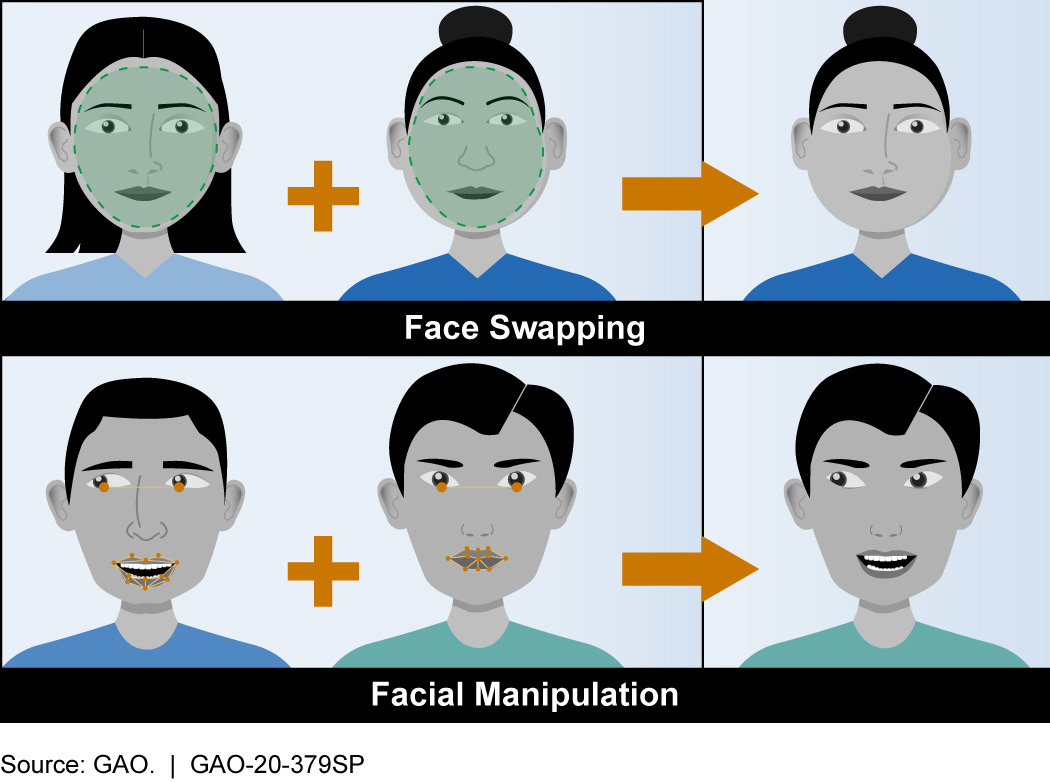
\includegraphics[width=0.9\textwidth]{images/704754.png}  
    \caption{Illustrations of face swapping and facial manipulation (source: gao.gov)}  
    \label{figure:deepfakes}  
\end{figure}  

%
% Tracking incidents
%
Tracking social engineering incidents can be accomplished by counting incident occurrences or by calculating the total cost of all incidents annually~\citep{ibm_Cost_Data_Breach_Report_2024}. Not all organizations report their social engineering and other cybercrime-related incidents, but very good estimates of the prevalence of these attacks can be gained from data that is gathered by various cybercrime-specialized public and private organizations. Their research is published in reports such as the \textit{Internet Crime Report}~\citep{fbi_Internet_Crime_Report_2023}, the \textit{Cost of a Data Breach Report}~\citep{ibm_Cost_Data_Breach_Report_2024}, the \textit{Data Breach Investigations Report}~\citep{verizon_Data_Breach_Investigations_Report_2024} and the \textit{Threat Landscape}~\citep{eniza_Threat_Landscape_2024}. 




Organizations can thus assess the effectiveness and impact of their new policies, software upgrades, and cultural changes by monitoring incident statistics, particularly incident-related annual costs. These costs include detection, investigation and recovery, and any loss of sales, customers and data. %The annual cybersecurity costs related to social engineering are the primary metric examined in this thesis.






%
% AI threat 
%
The dynamic nature of AI-driven social engineering poses a significant challenge for traditional cybersecurity frameworks, which often rely on static defenses and predefined patterns of attack~\citep{fakhouri_AI_Driven_Solutions_SE_Attacks_2024}. As generative AI technologies advance, their application in crafting personalized and convincing social engineering attacks becomes increasingly evident~\citep{blauth_AI_Crime_Overview_Malicious_Use_Abuse_2022}. This new capability not only enhances the likelihood of success but also complicates the detection and mitigation of such threats~\citep{mirsky_Threat_Offensive_AI_Organizations_2023}.











\section{Open-source intelligence}
\begin{comment}
Some case studies highlighting the use of OSINT in real-world social engineering incidents?
\end{comment}

Social engineering attacks begin with the gathering of data. In cybersecurity, publicly available information is known as \textbf{open-source intelligence}~\citep{hadnagy_Social_Engineering_The_Science_2018}. This practice involves collecting intelligence from sources that are publicly accessible, such as the target organization's website, employees' social media profiles, or other public records. Threat actors are increasingly utilizing platforms such as LinkedIn, Facebook, and X (formerly Twitter) to gather information about their victims~\citep{fakhouri_AI_Driven_Solutions_SE_Attacks_2024}.

Various online tools have been created for the purpose of gathering intelligence on an individual or an organization~\citep{mirsky_Threat_Offensive_AI_Organizations_2023}. They often offer automated forensic gathering and are able to visualize the found data, making it easier to identify exploitable patterns and connections. Many of these tools are adapting to use powerful AI technologies as well~\citep{wang_Defining_Social_Engineering_2020}.

Threat actors are also able to utilize sites like the Internet Archive and specific web searching features such as Google’s cache to find websites and other material that is no longer accessible via simple web search queries. Bots can be used to download social media posts at frequent intervals in case the target organization makes a mistake in one of their social media posts and deletes it promptly.

Lastly, open-source intelligence, as the name implies, does not contain intelligence gathered using any of the social engineering tactics discussed in the next chapter, such as calling customer support and asking for personnel information~\citep{hadnagy_Social_Engineering_The_Science_2018}. Open-source intelligence-gathering practices should not leave any traces behind.





\section{Generative AI}
\begin{comment}
\end{comment}

Artificial intelligence (\textit{AI}) encompasses the development of algorithms designed to automate complex tasks ~\citep{mirsky_Threat_Offensive_AI_Organizations_2023}. Currently, the most prevalent type of AI is machine learning, which enables systems to enhance their performance as they gain experience~\citep{fakhouri_AI_Driven_Solutions_SE_Attacks_2024}. Deep learning, a subset of machine learning, employs extensive artificial neural networks as predictive models~\citep{goodfellow_Generative_Adversarial_Networks_2020}. The core idea behind AI is to enable machines to mimic human-like decision-making and thinking processes.


When AI is used to generate content, it is called \textbf{generative AI}~\citep{goodfellow_Generative_Adversarial_Networks_2020}. Unlike traditional AI, which follows programmed rules, generative AI utilizes machine learning to learn patterns from large training datasets to produce new or similar outputs, such as text, images, audio, and video.

Currently, the most prominent example of generative AI is ChatGPT, a chatbot released by OpenAI in 2022\footnote{https://openai.com/index/chatgpt (visited on 2024-08-19)}. While far from being the first~\citep{weizenbaum_ELIZA_1996}, this chatbot revolutionized how people use and interact with generative AI systems, reaching over 100 million users in just two months\footnote{https://explodingtopics.com/blog/chatgpt-users (visited on 2024-08-11)}. Built on the GPT (\textit{Generative Pre-trained Transformer}) architecture, ChatGPT is designed to understand and generate human-like text by predicting the next word in a sequence.

Another relevant generative AI technology for social engineering is DALL-E, which was released in 2021 and which was also developed by OpenAI\footnote{https://openai.com/index/dall-e-3/ (visited on 2024-09-19)}. This system generates images from textual descriptions, facilitating digital manipulation and the creation of misleading visuals. It enables the production of hyper-realistic images that can distort or shape public perception.
